% !Mode:: "TeX:UTF-8"
%!TEX program  = xelatex

%\documentclass{cumcmthesis}
\documentclass[withoutpreface,bwprint]{cumcmthesis}
\renewcommand{\arraystretch}{1}
%\usepackage{url}
\usepackage[colorlinks,linkcolor=black]{hyperref}
\usepackage{listings}
\usepackage{float} 
\usepackage{caption}
\title{基于动态规划及刚体模型的同心鼓协作策略分析}
\tihao{B}

\begin{document}
 \maketitle
 \begin{abstract}
	同心鼓协作模型是一种有利于增进团队凝聚力的活动,同时,其本质(多人合作以达到一定目标)有较为广泛的应用,例如:工业多悬链生产作业,农业晒秋等。因此,最优化此协作模型有一定的研究价值。
	
	本文主要运用动态规划的方法并建立刚体模型,以最小化每一成员的做功量为目标,优化此模型。通过分析系统变量(鼓的竖直方向的速度$v_i$,鼓与排球之间的距离$Y_i$)与决策变量(沿绳的的力$F_i$,绳与水平面夹角$\theta_i$)求解以时间划分阶段的动态过程。同时,考虑非理想化状态下,通过研究刚体模型,适当调整策略,以增加策略的泛用性。
	
	问题一是最优化问题。利用动量守恒定理分析碰撞位置后,基于给定的数值以及约束条件,将要求(使连续垫球次数尽可能多)转化为减少每位成员累积做功值。由于鼓的运动速度,加速度,位移等运动状态参数未知,我们将连续的变量位移离散化,并用状态转移方程组表示出此系统中鼓面与球的运动状况。选取力的大小及力的方向为决策变量,在此动态系统下累加求得平均做功值 W,采用遗传算法选取 W 最小化的情况下的动态系统,从而得到最佳策略。
	
	问题二是基于理想化模型的求解问题。据题目要求,可以默认队员仍然可以精确控制发力的角度。在合理范围内,为了简化模型,我们假设,队员在整个发力区间0-0.1s内始终控制绳与鼓面的夹角保持不变,即初始夹角。同时,我们根据刚体的性质,并结合平行轴定理,建立“二维圆盘模型”,积分计算转动惯量。由于距心相同的两个力矩可以按平行四边形法则合成,结合角位移与转动惯量等的关系,可以求得角位移。
	
	问题三是调整策略的问题。忽略问题一中理想模型的假设,考虑问题二中未精确控制用力大小及时机导致的鼓面倾斜状况。通过此种特殊情况的代入情况对问题一中的策略进行相应改进,从而使该模型更具有普适性。
	
	问题四是模型的代入问题,也可以看作系统优化设计问题。将问题场景中的数值代入由前三个问题所得出并完善的模型,求解对应其他参数的变化情况。\\
	\vbox{} 
\keywords{动态规划\quad 刚体的受力分析\quad 理想化模型\quad 遗传算法}
\end{abstract}
\newpage
\section{问题重述}
\subsection{问题背景与研究意义}
团队协作是指通过团队完成某项制定的事件时所显现出来的自愿合作和协同努力的精神。为了增加团队向心力,培养成员的合作意识,许多团队选择开展团队能力拓展项目。其中,“同心协力”(同心鼓)便是一种激励团队精神的活动。为了增进团队凝聚力,使得团队合作效益最大化,同心鼓活动的具体策略值得探索与研究。同时,此模型本质上可以被简化为一种多人协作以达到一定目标的模型,由此,可以应用于人们生活的方方面面。例如:在工业方面,工厂调用多自由度的多条悬链同步进行对生产运输系统的控制;在农业方面,农民在秋收时节,使用大型竹编簸箕,竹筛子,竹圆盘等抖动晾晒筛选玉米豆等农作物;在人际交往方面,人们为表达喜悦,经常模仿历史上耶稣复活的节日里的庆祝仪式,将事件主角抛向空中等。综上,建立同心鼓的策略模型并进行优化,具有很大的研究意义。
\subsection{问题的提出}
现有一个由排球,鼓,绳,队员组成的同心鼓系统。其中,项目所用排球的质量为0.27kg;鼓的质量为3.6kg,鼓面直径为0.4m,鼓身高度为 0.22m;绳系在鼓身正中间且呈均匀分布;项目开始时,球从鼓面中心上方0.4m处竖直落下。此项目的目标是使得队员连续颠球的次数尽可能多。\\
游戏的要求如下:
\begin{itemize}
	\item 队员握住绳子末端对鼓进行控制,游戏中不可接触鼓或绳子的其他位置。
	\item 队员人数不少于8人,相互之间的最小距离不得小于0.6m。
	\item 球被颠起的高度应距鼓面0.4m以上,否则项目停止。
\end{itemize}
针对此系统,题目给出以下几个问题:
\begin{enumerate}
	\item 在每个队员均可以精确控制用力方向、时机和力度的情况下讨论此理想化模型下团队的最佳协作策略;并求出此策略下颠球高度。
	\item 已知当队员的用力时机和力度不能精确控制时,鼓面会发生倾斜。设队员人数为8,绳长为1.7m。鼓面初始时刻是水平静止的,初始位置较绳子水平时下降0.11m。在此情况下,建立能够描述鼓面倾斜角度与队员发力时机和力度关系的模型;并分别求出题目给出的9种具体场景下鼓面的倾斜角度。
	\item 依据问题2所建立的模型调整优化问题1提出的策略。
	\item 在鼓面发生倾斜的情况下,设队员人数为10,绳长为2m。球的反弹高度为0.6m,相对于竖直方向产生1度的倾斜角度,且倾斜方向在水平面的投影指向某两位队员之间,与这两位队员的夹角之比为1:2。为了将球调整为竖直状态弹跳,求得在可精确控制条件下所有队员的发力时机及力度,并分析在实际中此调整策略的实施效果。
\end{enumerate}

\section{问题分析}
\subsection{问题总分析}
\begin{center}
	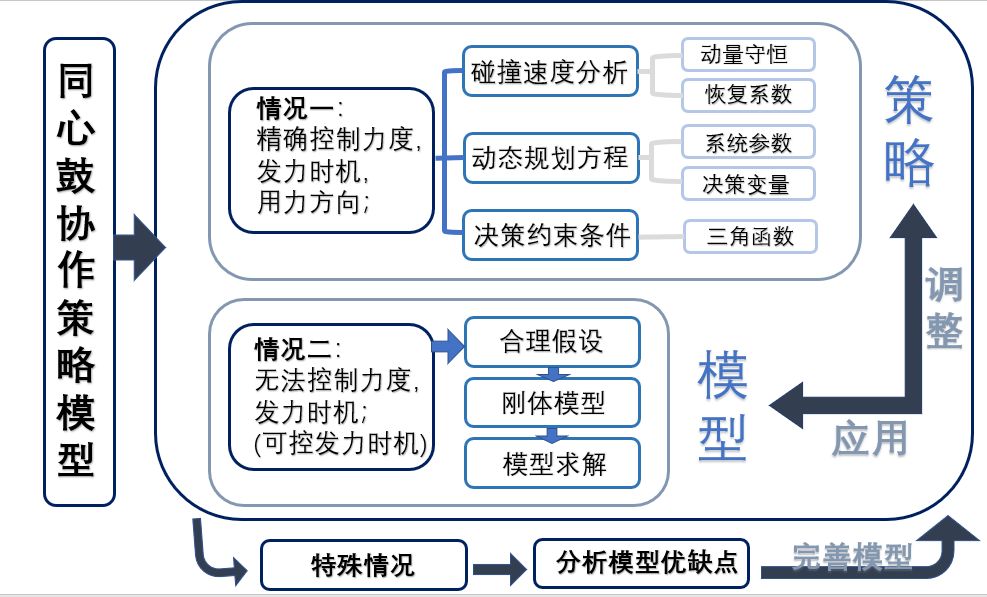
\includegraphics[scale = 0.57]{lc.png}
\end{center}

\subsection{问题一的分析}
问题一是最优化问题。给定了球的质量,鼓的质量,球的初始高度;约束条件有:两队员之间的距离不得小于0.6m;队员总人数不少于8人;球每次离开鼓面高度高于0.4m。本题要求使连续垫球次数尽可能多,由于鼓可保持水平且作用其的力可被精确控制,本题可理解为目标使队员在能量耗尽前能连续垫球的次数最多,从而可以将优化目标转化为最小化每次垫球所做的功。由于鼓的运动速度,加速度,位移等运动状态参数为未知,我们将连续的位移离散化,并用状态转移方程组表示出鼓面的运动速度 v 以及球和鼓面的距离 Y。该状态转移方程组选取鼓面的移动速度与球和鼓面的距离为决策变量,并在此动态系统下求得做功值 W,并采用遗传算法选取 W 最优的情况下的动态系统,从而得到最佳策略。
\subsection{问题二的分析}
问题二是基于理想化模型的求解问题。区别于问题一设定的理想化模型(每个队员可以精确控制用力方向,时机和力度),问题二更加趋近于现实化情况:队员的发力时机和力度不再做到精确控制。然而,与问题一相比较,可发现此问题并没有限定队员的发力角度,由此可以默认队员仍然可以精确控制发力的角度。在合理范围内,为了简化模型,我们假设,队员在整个0.1s内始终控制绳与鼓面的夹角保持不变,即初始夹角 $arcsin\frac{0.11}{1.7}$。

同时,我们根据刚体的性质,建立“二维圆盘模型”计算转动惯量。首先,假设鼓为一个质量均匀分布的实心圆柱体。此圆柱体于通过其质心,与其几何轴垂直的轴转动。由此,可以将此圆柱体沿垂直于几何轴的平面无数等分。取一个厚度为极小量$\delta h$的圆盘,由于此柱体的密度$\rho$处处相等,在圆柱体的高H上积分,结合平行轴定理,可得整个圆柱体的转动惯量 I。由于矩心相同的两个力矩可以按平行四边形法则合成,再结合角位移,角加速度,转动惯量,时间的关系,可以求得角位移。
\subsection{问题三的分析}
问题三是调整策略的问题。即忽略问题一中理想模型的假设,考虑问题二中未精确控制用力大小及时机导致的鼓面倾斜状况。通过此种特殊情况的代入对问题一中的策略进行相应改进,从而使该模型更具有普适性。研究认为可以适当增加k值采用近似,减小误差或者采用泛函分析的方法。
\subsection{问题四的分析}
问题四是模型的代入,可以看作系统优化设计问题。将问题场景中的数值代入由前三个问题所得出的模型,已知了球的反弹高度和初始首次反弹状态,也确定了人数,绳长两个参数,即修改球反弹的倾斜角度,求解对应其他参数的变化情况。

\section{模型的假设}
\subsubsection{第一部分:球与鼓的碰撞模型}
\begin{itemize}
	\item 空气阻力及一切摩擦可忽略不计。
	\item 鼓面任意时刻始终保持水平。
	\item 每个参与者拉绳的力大小,方向,用力时机完全相同。
	\item 绳为理想模型,质量可忽略。
	\item 球为质点模型。
\end{itemize}

\subsubsection{第二部分:鼓的倾斜模型}
\begin{itemize}
	\item 使参与者保持每根绳子与鼓面的夹角任意时刻不变。
	\item 鼓可视为质量均匀分布的圆柱体。
	\item 参与者对绳子施加的力的大小在0.1秒内恒定不变。
	\item 球从初始位置下落到第一次碰撞后进入可持续周期。
\end{itemize}

\section{符号说明}
\begin{table}[H]
	\centering
	\caption{碰撞速度模型}
	\begin{tabular}{ c c c c c}
	\hline
	 符号 & 符号说明 & & 符号 & 符号说明\\ 
	\hline
	 m_1 & 球的质量 &  & m_2 & 鼓的质量\\  
	 v_0' & 第一次碰撞前球的速度 & & v_1' & 第一次碰撞前鼓的速度\\ 
	 v_0 & 碰撞后球的速度 & & v_2 & 碰撞后鼓的速度\\
	 v_0 & 第二次及以后碰撞前球的速度 & & v_1 & 第二次及以后碰撞前鼓的速度\\
	 x & 鼓面初始位置和碰撞位置的距离 & & n & 参与项目的人数\\
	 \overline{P} & 每次运动的总平均功率 & & W & 每次运动的总做功\\
	 e & 恢复系数\\
	\hline
	\end{tabular}
\end{table}	

\begin{table}[H]
	\centering
	\caption{球与鼓运动时的动态系统}
	\begin{tabular}{ c c c c c}
	\hline
	 符号 & 符号说明 & & 符号 & 符号说明\\ 
	\hline
	 d & 鼓面最低与最高点之间的距离 &  & \Delta x & 鼓面在极短时间内的位移\\  
	 \Delta t & 极短时间 & & g & 重力加速度\\ 
	 v & 鼓面的运动速度 & & Y & 球与鼓面的距离\\
	 a & 鼓面的运动加速度 & & F & 绳对鼓面的作用力(方向沿绳)\\
	 \theta & 绳与水平面的夹角 & & W & 人对鼓做的功\\
	 k & 一个尽可能大的整数 & & n & 参与项目的人数\\
	\hline
	\end{tabular}
\end{table}

\begin{table}[H]
	\centering
	\caption{人数n的评估模型}
	\begin{tabular}{ c c c c c}
	\hline
	 符号 & 符号说明 & & 符号 & 符号说明\\ 
	\hline
	 l & 绳子的长度 &  & n & 参与项目的人数\\  
	 \theta & 绳与水平面的夹角 & & d & 两人之间的距离\\
	\hline
	\end{tabular}
\end{table}

\begin{table}[H]
	\centering
	\caption{鼓面倾斜模型}
	\begin{tabular}{ c c c c c}
	\hline
	 符号 & 符号说明 & & 符号 & 符号说明\\ 
	\hline
	\beta & 角加速度&  & I & 转动惯量\\  
	 r & 鼓面半径 & & m & 鼓的质量\\
	\rho & 鼓密度 & & \Delta{h} & 鼓的小段高度\\
	 H & 鼓身长度 & & \alpha & 角位移\\
	\hline
	\end{tabular}
\end{table}

\section{模型的建立与求解}
\subsection{问题一:碰撞模型}
\subsubsection{碰撞速度模型}
在每个人都可以精确控制用力方向,时机,力度时,要使连续垫球的次数尽可能多,我们最小化抛球的平均总功率从而达到最佳策略。球与鼓面碰撞前后的运动状态如下图所示:
\begin{figure}[H]
	\centering
	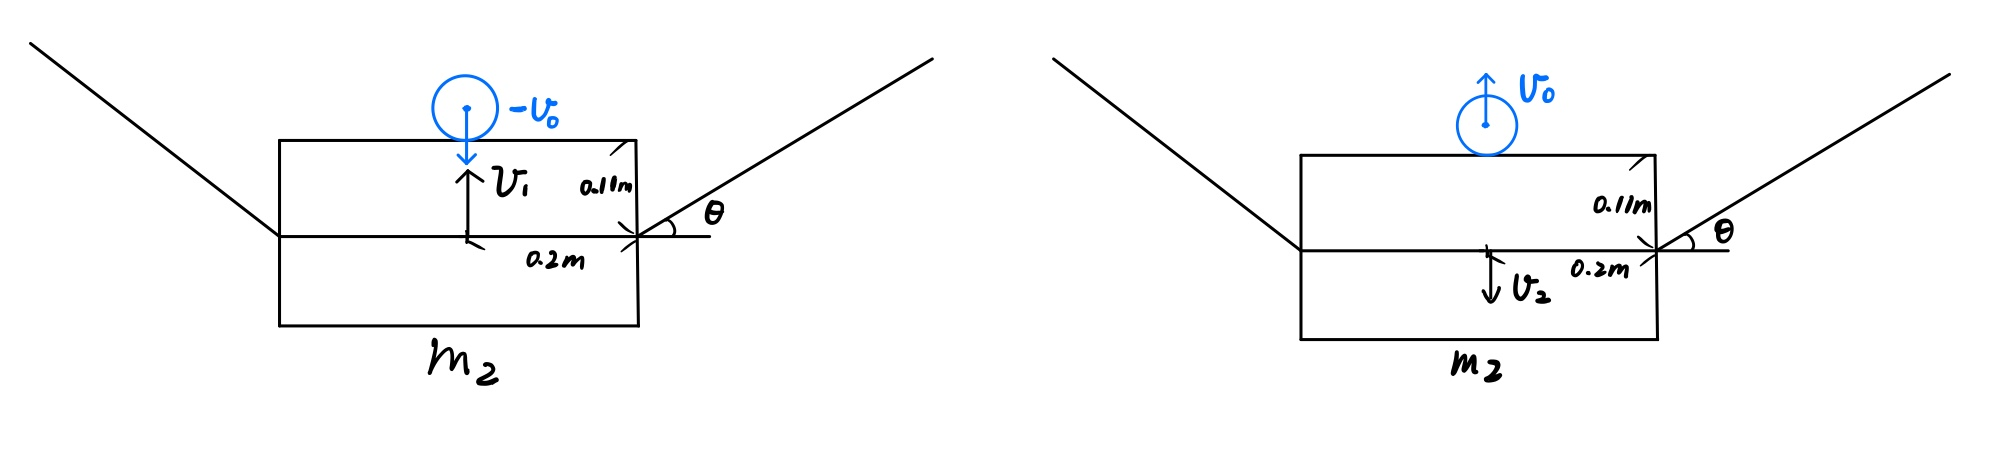
\includegraphics[scale = 0.23]{IMG_0011.jpg}
	\caption{球与鼓面碰撞前后的状态示意}
\end{figure}

\begin{center}
	W = $\frac{1}{2}$m_2v_1^2 - \frac{1}{2}m_2v_2^2\\
	$$min\ \overline{P} = \frac{W}{2t} = \frac{\frac{1}{2}m_2\left(v_1^2 - v_2^2\right)}{\frac{v_0}{g}} = \frac{m_1\left(v_1 - v_2\right)g}{2}$$
\end{center}
所以我们将优化目标转化为使$\left(v_1 - v_2\right)$最小。由动量守恒定理我们可以联立方程组:
\begin{equation}
	\begin{cases}
		v_0 + v_1 = e (v_0' + v_1')\\
		-m_1v_0' + m_2v_1' = m_1v_0 - m_2v_2\\
		-m_1v_0 + m_2v_1 = m_1v_0 - m_2v_2 \\
	\end{cases}	
\end{equation}
通过求解方程组,我们得到等式:
\[\left(m_1 - m_2\right)\left(v_2 - v_1'\right) = 0 \]
由于球与鼓的质量不相同,可以得到: \[v_2 \not= v_1'\]从而推得小球每次弹起的最高点高度相同,由于球的弹起高度须大于0.4m,从而推得每次碰撞前,鼓面需调整至鼓的初始位置之下$\left(x <= 0\right)$。

\subsubsection{球与鼓运动时的动态系统}
要达到垫球的最优策略,即垫球次数尽可能多,我们可以认为在团队力量耗尽前,球下落并从鼓面弹起是一个周期性运动。在固定团队总做工的情况下,减少在球的一个运动周期内做的功的数量即可得到最优策略。该情景拥有最优子结构特征;并且优化的子问题与母问题重叠;该优化过程存在边界:球与鼓面的距离减少至0,故应采取动态规划方法求解最优策略。

如下图所示,我们将该连续的过程离散化,再采取遗传算法求得最小功。取一个较大整数k,将鼓面从最低至最高点的过程分为k个阶段,每段位移表示为$\Delta x$,每段时间表示为$\Delta t$。i 表示第 i 个阶段系统的运动状况。

\begin{figure}[H]
	\centering
	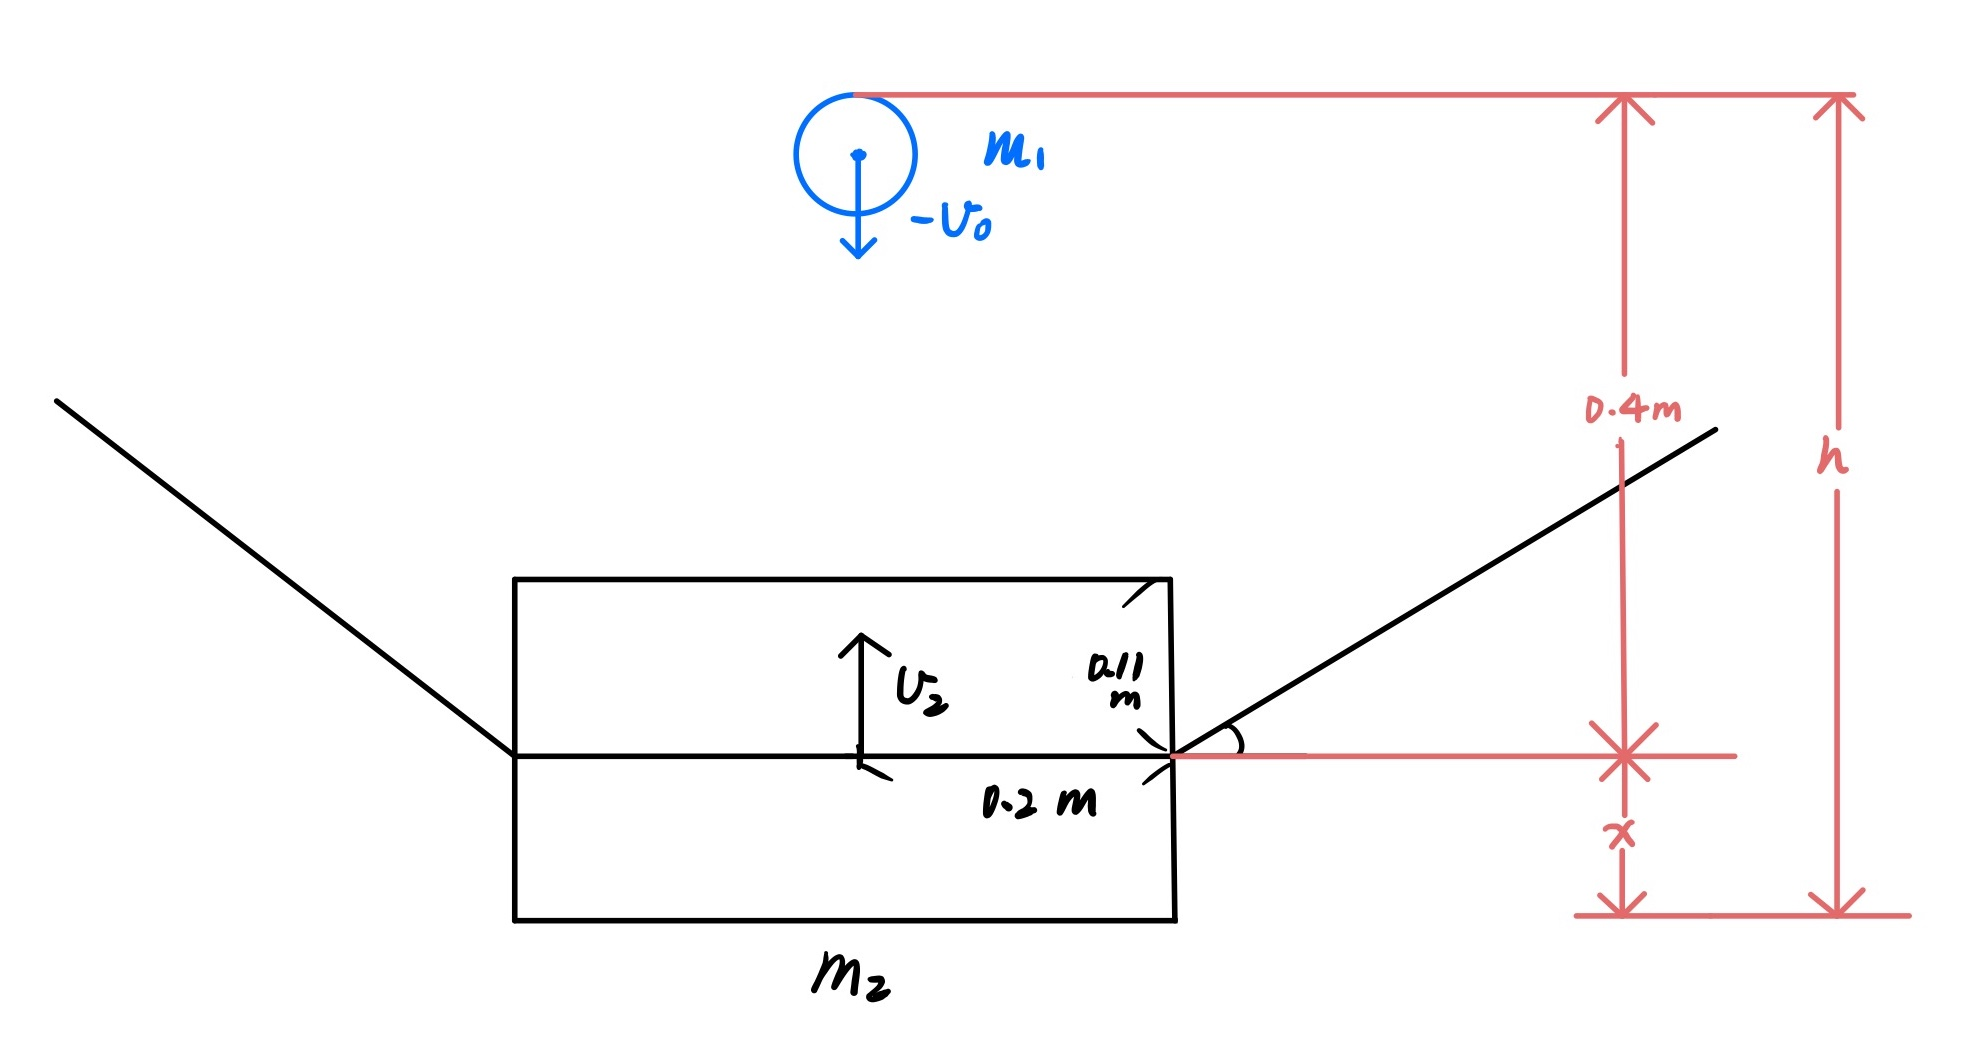
\includegraphics[scale = 0.20]{IMG_0014.jpg}
	\caption{离散化的球与鼓面运动示意图}
\end{figure}

我们选取鼓面在 i+1 时刻的运动速度$\left(v_{i+1}\right)$和鼓面与球在第 i+1 时刻的距离 $\left(Y_{i+1}\right)$为该动态系统的特征并联立方程组:

\begin{equation}
	\begin{cases}
		v_{i+1} = v_i + a_i \Delta t\\
		Y_{i+1} = Y_i - \Delta x - \frac{1}{2}g\left(\Delta t\right)^2
	\end{cases}
\end{equation}
将鼓面在极短的时间内的运动视为匀加速直线运动,我们可以将$\Delta x$表示为:
\[\Delta x = \frac{d}{k} = v_i\Delta t + \frac{1}{2}a_i\left(\Delta t\right)^2 = \Delta x\]
基于对鼓的受力分析,我们可以得到鼓面在 i 时刻的加速度:
\[nF_i sin\theta_i - m_2g = m_2a_i\]
\[a_i = \frac{nF_i sin\theta_i - m_2g}{m_2}\]
将以上等式带入状态转移方程组,我们将方程组优化成以下表达形式:
\begin{equation}
	\begin{cases}
		v_{i+1} = f\left(v_i, Y_i, F_i\right)\\
		Y_{i+1} = g\left(v_i, Y_i, F_i\right)
	\end{cases}
\end{equation}
通过变量的代入与化简,我们可以将$v_{i+1}, Y_{i+1}$转化成关于$v_i, Y_i, F_i$ 的函数。假设 q 时刻(1 $<$ q $<$ k)鼓面与球碰撞,此之前绳的力对鼓的做工可表示为:
\[\sum_{i = 1}^qW_i = \sum_{i = 1}^qnFi\Delta x sin\theta_i\]

\subsubsection{对于参与人数n的评估模型}
由情景可知,参与队员人数不得少于 8 人。如果考虑每位队员能做的功是有限的,并以做工少,队员省力为最优策略目标,则可认为参与人数越多越优。但由于两队员之间的距离 d 最小不得小于0.6m, 如下图所示:
\begin{figure}[H]
	\centering
	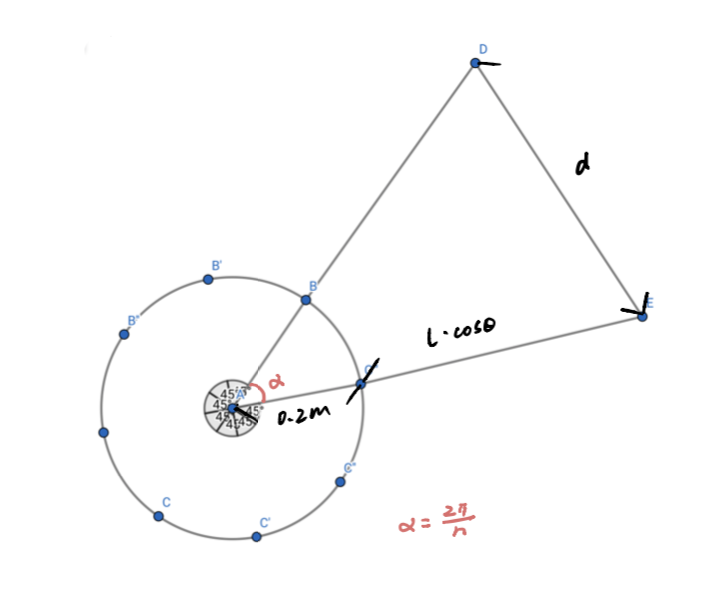
\includegraphics[scale = 0.75]{N.png}
	\caption{两队员与中心连线三角形示意}
\end{figure}
由余弦定理可得如下等式:
\[2\left(0.2 + lcos\theta\right)^2cos\frac{2\pi}{n} = 2\left(0.2 + lcos\theta\right)^2 - 0.6^2\]
由此等式解得 n 并得出参与人数 n 的上限值:
\[n = \frac{2\pi}{arccos\frac{\left(0.2 + lcos\theta\right)^2 - 0.18}{\left(0.2 + lcos\theta\right)^2}}\]

\subsection{问题二:倾斜模型}
本部分是探讨队员发力时机与力度的误差导致鼓面出现倾斜的情况,我们使用动作误差产生的转动惯量得出鼓在该时段的角加速度,由于线与鼓面的角度保持不变,倾斜过程可视为匀加速运动。
\begin{figure}[H]
	\centering
	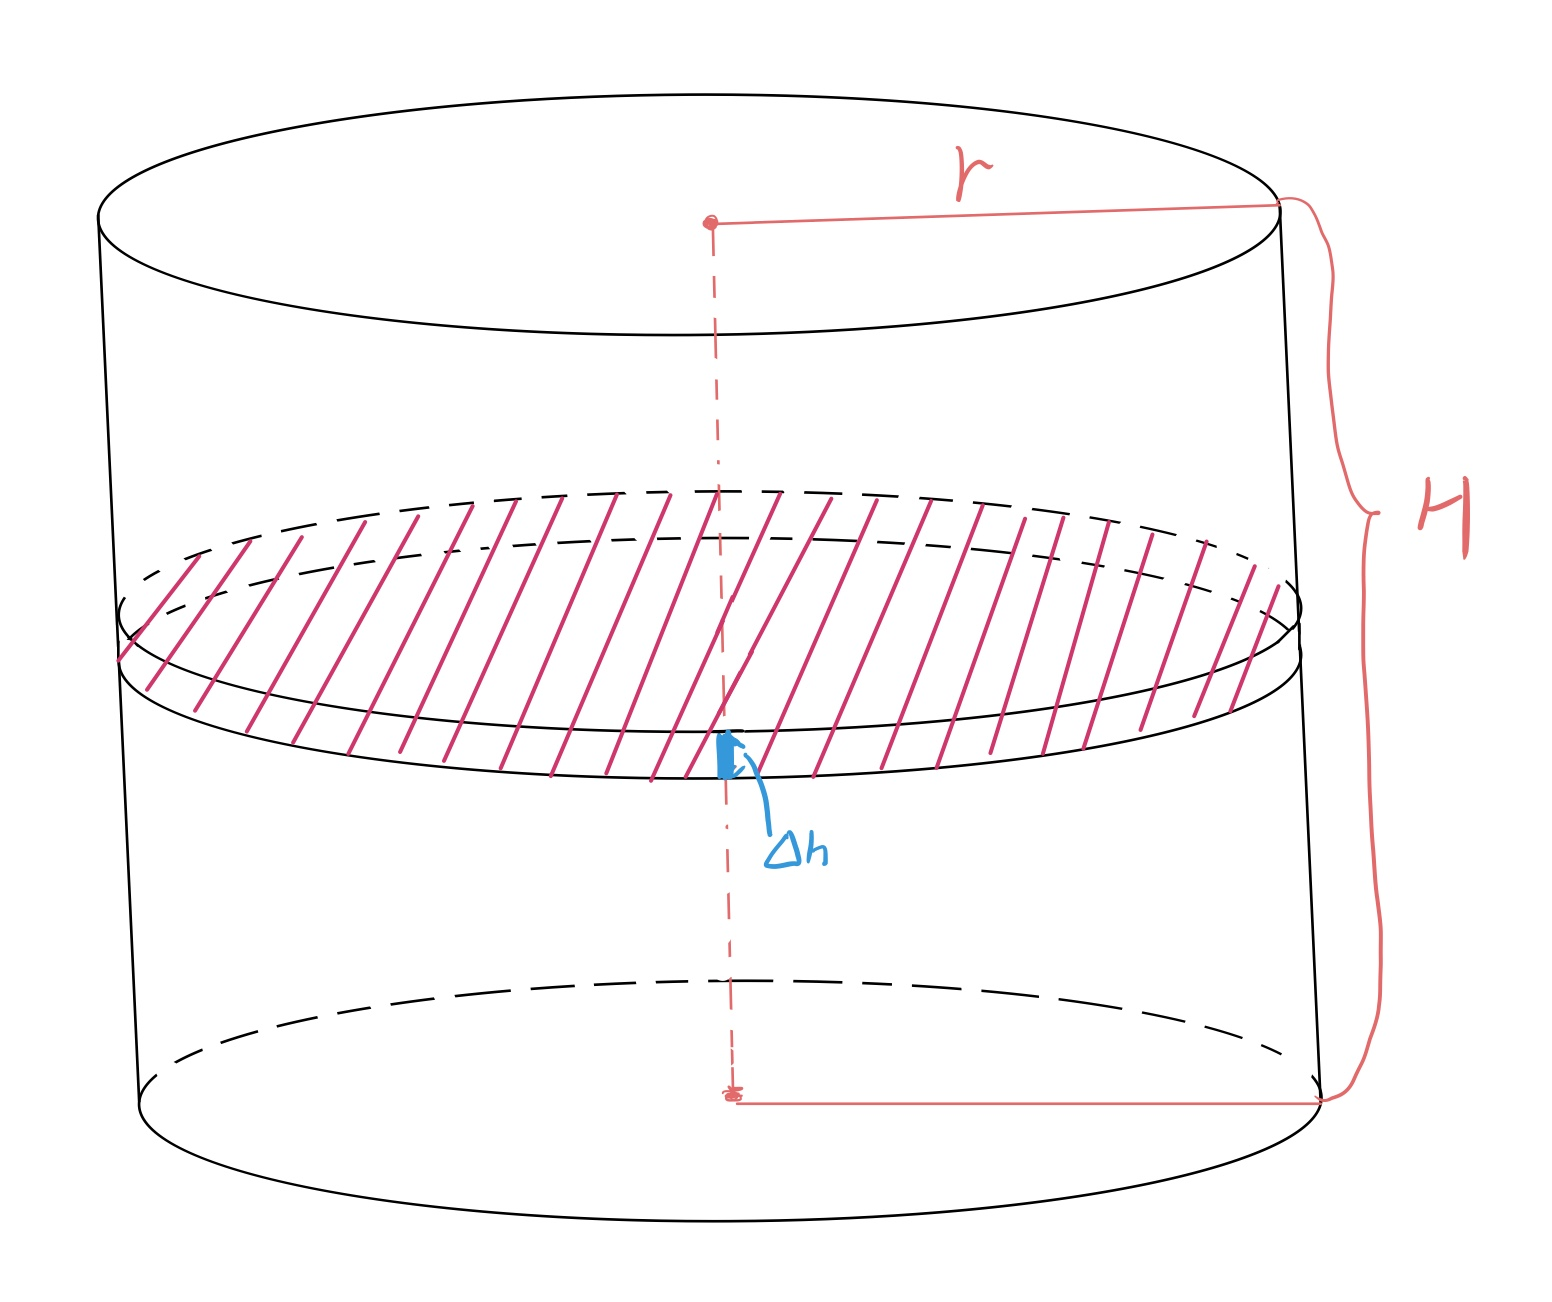
\includegraphics[scale = 0.14]{IMG_0018.jpg}
	\caption{转动惯量的积分示意图}}
\end{figure}
转动惯量是刚体绕轴转动时惯性(回转物体保持其匀速圆周运动或静止的特性)的量度。按如上图所示以 h 为变量积分,转动惯量的表达式:
\[I = \rho\pi{r^2}\int_{-\frac{h}{2}}^{\frac{h}{2}}\left(\frac{r^2}{4} + h^2\right)dh\]
鼓的密度可表示为:
\[\rho = \frac{m}{\pi{r^2L}}\]
由此可将转动惯量化简为:
\[I = \frac{mr^2}{4} + \frac{mL^2}{12}\]

\subsubsection{施力不均时鼓面的倾斜模型}
第一种情况是:各队员发力时机相同,但有队员发力大小与其他队员不同,此时由于情景中队员握住绳子末端均匀站立在鼓周围,对称的力可相互抵消,从而简化成一个外力,如下图所示:
\begin{figure}[H]
	\centering
	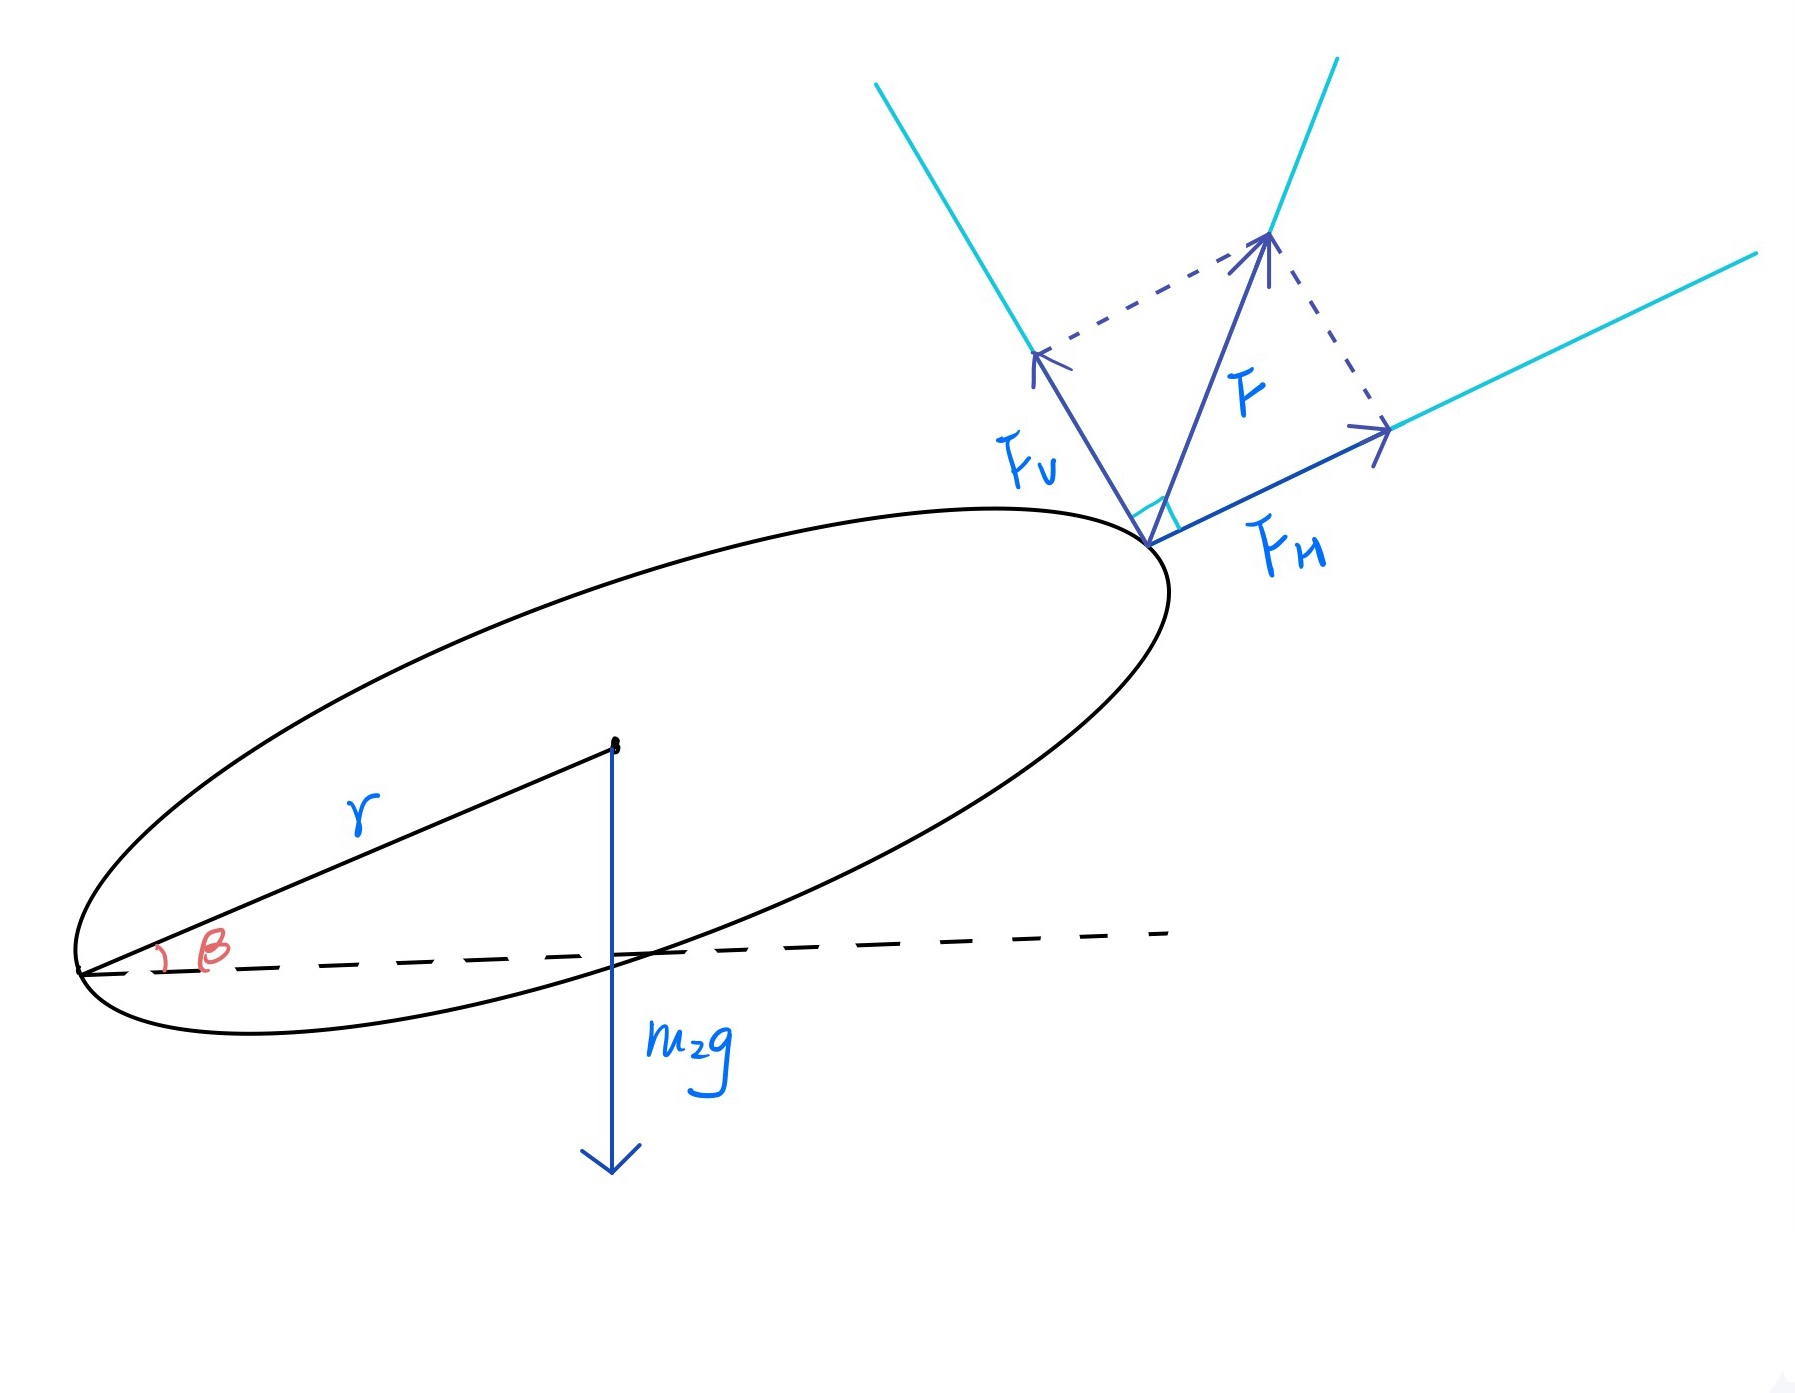
\includegraphics[scale = 0.14]{IMG_0017.jpg}
	\caption{力抵消后的外力示意}
\end{figure}
若有两位成员发力大小不同于其他成员,情况如下图所示:
\begin{figure}[H]
	\centering
	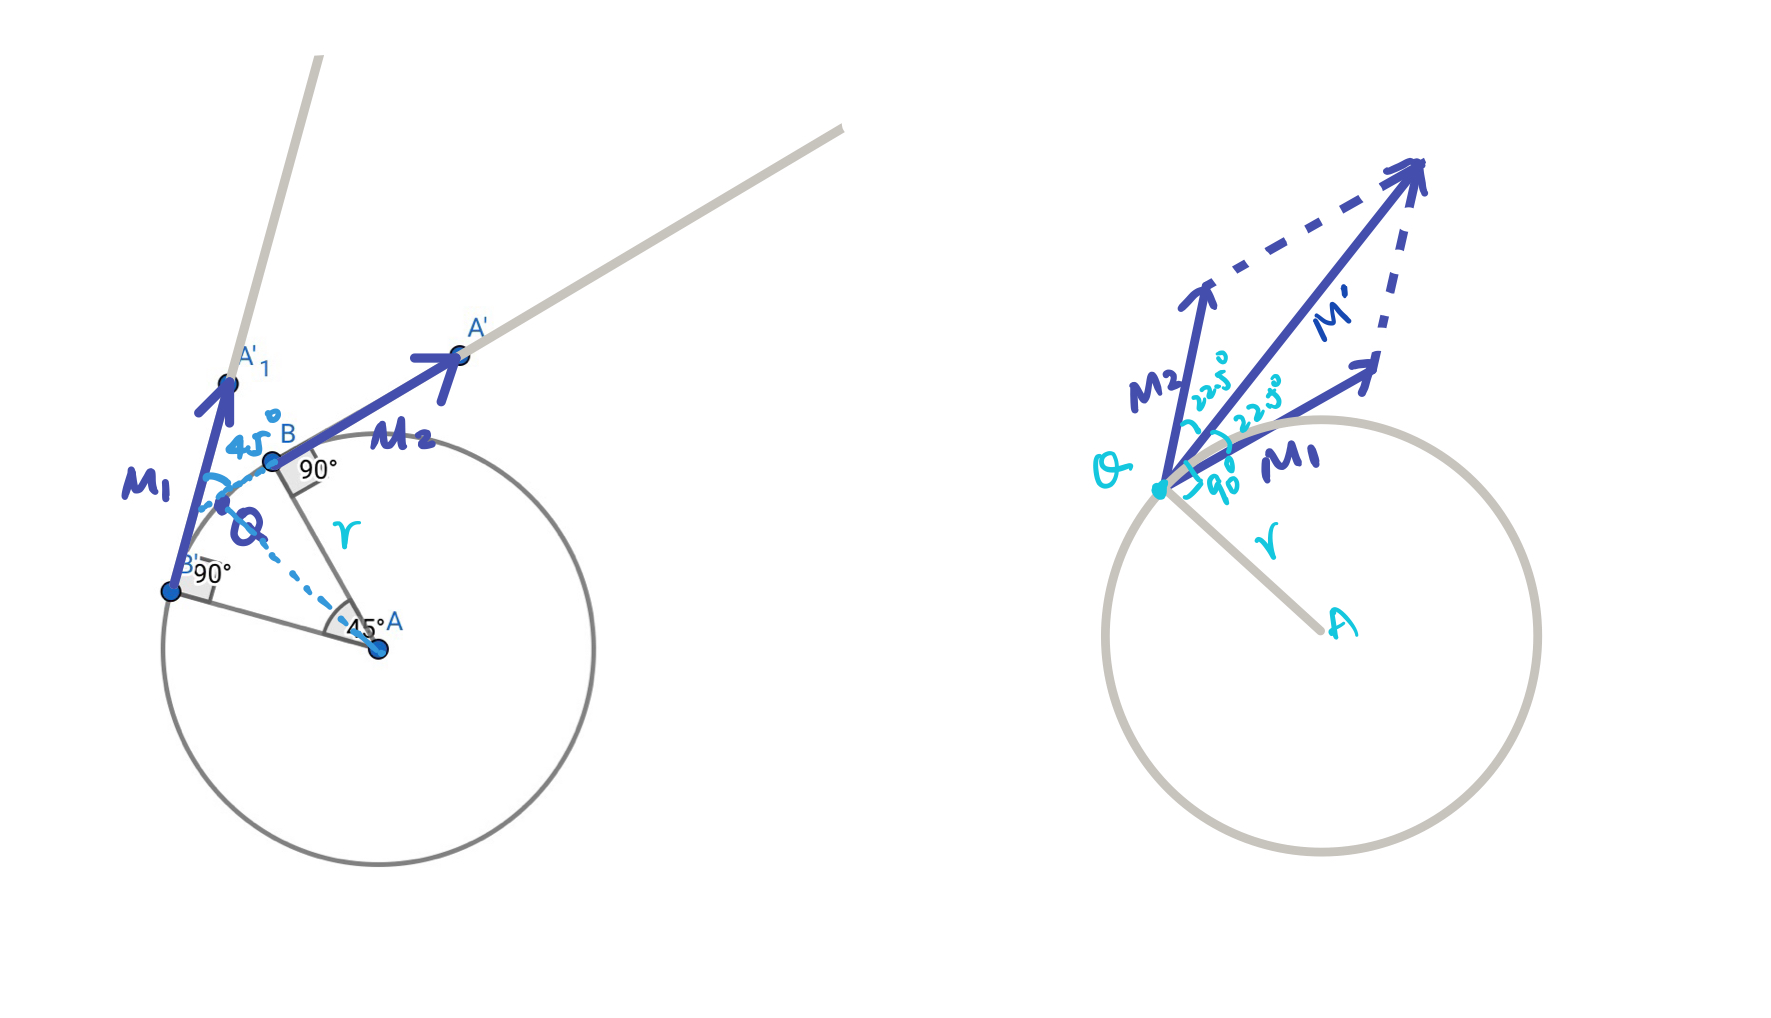
\includegraphics[scale = 0.28]{IMG_6F4646E3A079-1.jpeg}
\end{figure}
已知力与角加速度与转动惯量之间的关系:
\[Fsin\theta{r} = I\beta\]
从而可依据 F 的情况求得 $\beta$,已知加速时间为 t,由角度的匀加速运动公式可得出角度变化:
\[\alpha = \frac{1}{2}\beta{t}^2\]

\subsubsection{施力时机误差时鼓面的倾斜模型}
当出现成员发力时机出现误差(提前发力)时,在该成员提前发力的时间内,鼓仅受到来自出现误差成员方向的拉力 F,
利用 F 可由以下等式解得$\beta$:
\[Fsin\theta{r} = I\beta\]
小段时间后,当其余成员发力时,鼓面变成角速度为匀速$\omega$的旋转,已知运动时间为t,角度变化可表示为:
\[\omega = \beta{t}\]
\[\alpha = \frac{1}{2}\beta{t^2} + \omega{t}\]

\subsubsection{施力时机与施力大小均出现误差的模型}
绳子上的力只有垂直于鼓面的方向上才会产生力矩。现只考虑绳上的力在垂直方向上的分量所构成的平行力系,则平行力系的合力: 
\[F_R = \sum_{i = i}^nF_i\]
以圆盘(鼓面)为参照系,平行力系中心的坐标可表示为:
\[x_c = \frac{\sum_{i=1}^nF_ix_i}{\sum_{i = 1}^nF_i}\]
\[y_c = \frac{\sum_{i=1}^nF_iy_i}{\sum_{i = 1}^nF_i}\]
\[z_c = 0\]
力矩可表示为:
\[M = \sqrt{{x_c}^2 + {y_c}^2}F_R\]
可得到角加速度:
\[\beta = \frac{M}{I}\]
\subsubsection{代入结果}
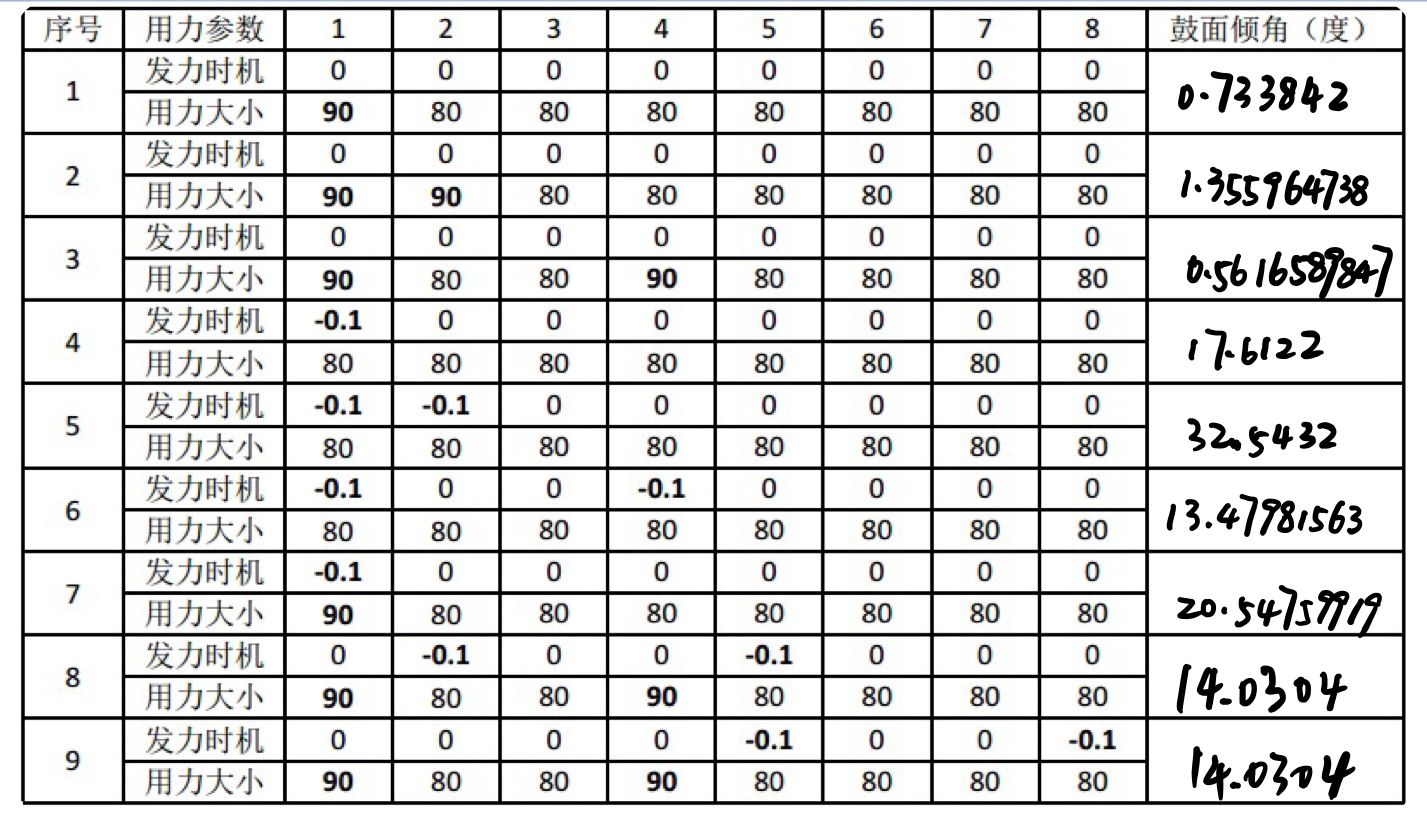
\includegraphics[scale = 0.33]{IMG_31CE30BB597B-1.jpeg}

\subsection{问题三:模型的改进}
问题一中的策略需要调整。由于在问题一的模型中,队员精确控制发力时机,力度与方向,鼓并不会发生转动而可以保持一直平动或静止,因而将位移k段等分(k为常数),取离散数值时,可以假设在状态方程组中:
\begin{equation*}
	\begin{cases}
		v_{i+1} = f\left(v_i, Y_i, F_i\right)\\
		Y_{i+1} = g\left(v_i, Y_i, F_i\right)
	\end{cases}
\end{equation*}
对于每一个队员来说,默认$F_i, \theta_i$ 在一定的第i段时,为相同的数值,从而累加得出做的总功:
\[\sum_{i = 1}^qW_i = \sum_{i = 1}^qFi\Delta x sin\theta_i\]
然而,当发力时机与力度不能够精确控制,鼓不但发生平动并且伴随转动,在便不适合默认每个队员沿绳施加的拉力$F_i$相等,从而导致目标函数W出现偏差。因此,需要调整。\\
调整策略:\\
1.取尽可能大的整数k值。当k尽可能大时,鼓在极短位移$\Delta{x}$做匀加速直线运动,此段中所受力$F_i$可以近似为相等,由此累加得到的W误差较小(但此种情况在极端情况下仍可能有误差)。\\
2.采用泛函分析的方法。在此道题目中,由于在进入周期后,排球始终重复做竖直上抛以及自由落体运动,因此只需研究鼓的运动。可综合运用函数观点,代数理论来研究未知函数加速度$a(·)$在无限维向量空间上的泛函,在一定约束条件$g_i(a(·))$下,对每位成员所作总功 $W (a(·))$ 采取适合的算法求取最小值。

\section{模型的评价与优化措施}
\subsection{模型的优点}
\begin{itemize}
	\item 本文将实际游戏中相对复杂的协作问题转化为最优化功率的问题,使用状态转移方程,使问题具体化。
	\item 本文将鼓与小球分隔分别进行讨论,并将绳上的力沿适当平面垂直分解,并且合理构造相对理想化的模型(转化为质点,刚体等),使问题简单化。
	\item 本文采用离散化变量的算法,在不改变不改变数据相对大小的条件下,对数据进行相应的缩小,将无限空间中有限的个体映射到有限的空间中去,简化了模型,提高了算法的时空效率,使其形式变得更加优美,方便求解。
	\item 本文除了必要假设以及简化,其余结果基本由严格计算获得,所以模型之中系统误差来源比较单一,泛用性较强。
	\item 基于离散化变量的状态转移方程模型符合实际游戏协作的过程与协作者的心理,经数据检验之后,模型的实用性和算法的有效性较高。
\end{itemize}

\subsection{模型的缺点}
\begin{itemize}
	\item 本文为简化模型,未考虑空气阻力与可能产生的摩擦力的影响。
	\item 本文默认所有游戏参与者具有相同无差的特质(对力度,方向,实际的控制;反应时间等),与实际有一定差别。
	\item 本文设计的同心鼓协作模型是基于离散化的变量基础之上的,假设每一段极小竖直位移中同心鼓做匀加速直线运动的,与实际中连续变化的变加速运动有一定偏差。
\end{itemize}

\subsection{模型的优化措施}
\begin{itemize}
	\item 针对连续变化的运动进行求解,使用泛函分析的方法,在多维空间中讨论同心鼓的运动情况,尽力消除离散化变化带来的近似误差。
	\item 可适当考虑空气阻力等其他因素对系统造成的影响。
	\item 采用模拟仿真的方法,使模型更加贴合实际情况,数据表现得更加直观。
\end{itemize}

\newpage
\section{参考代码}
\begin{itemize}
	\item 遗传算法 Python\\
	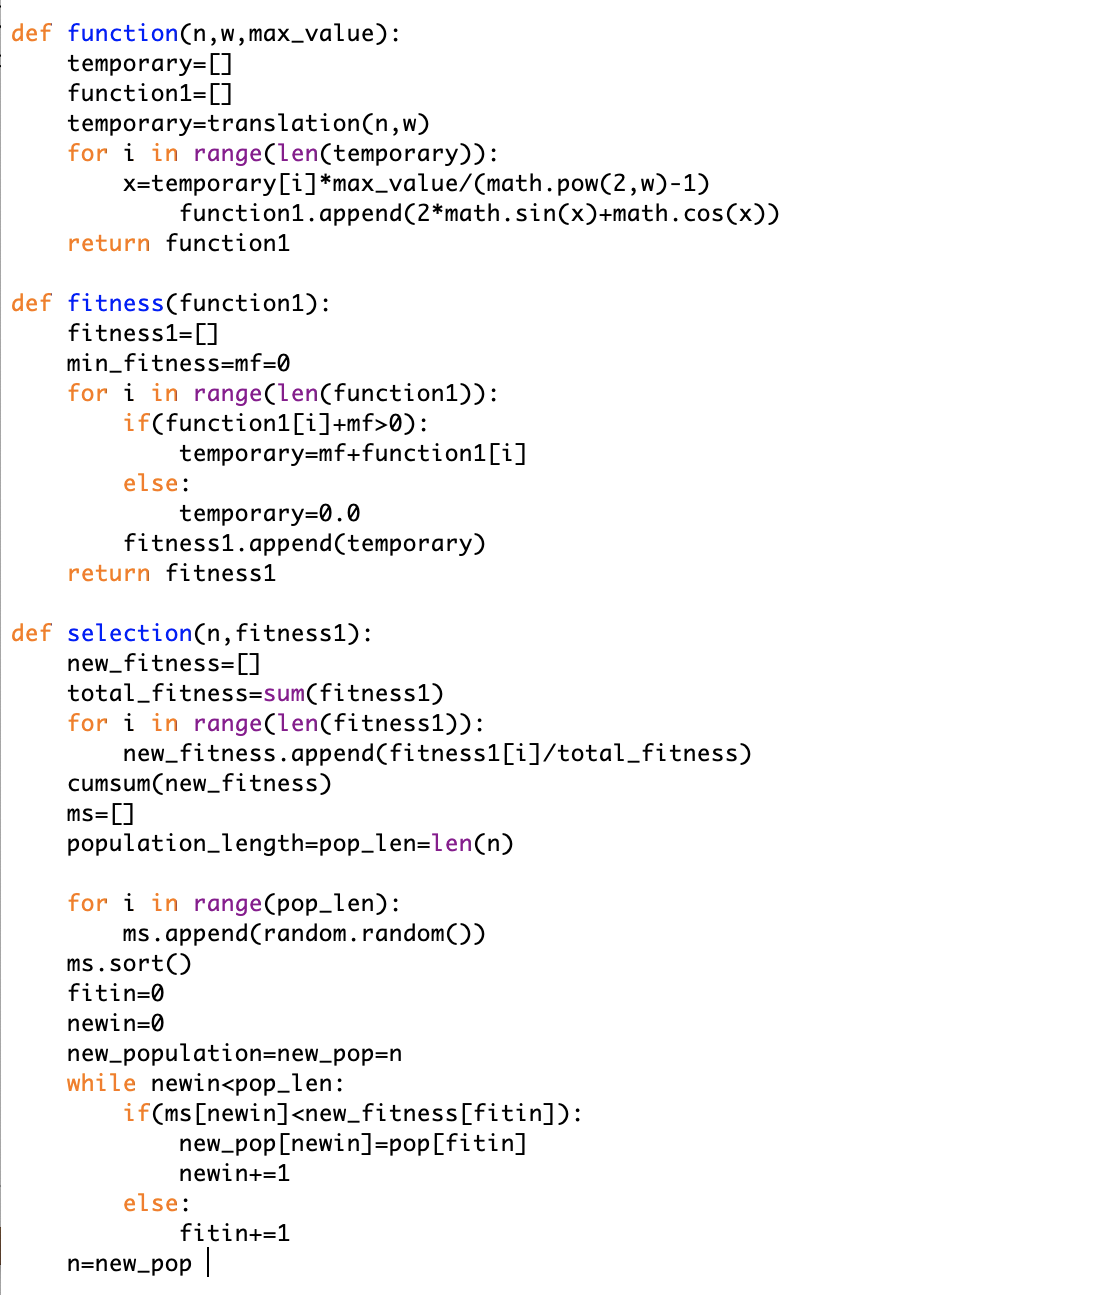
\includegraphics[scale = 0.6]{code1.png}
	\item 动态规划 Python\\
	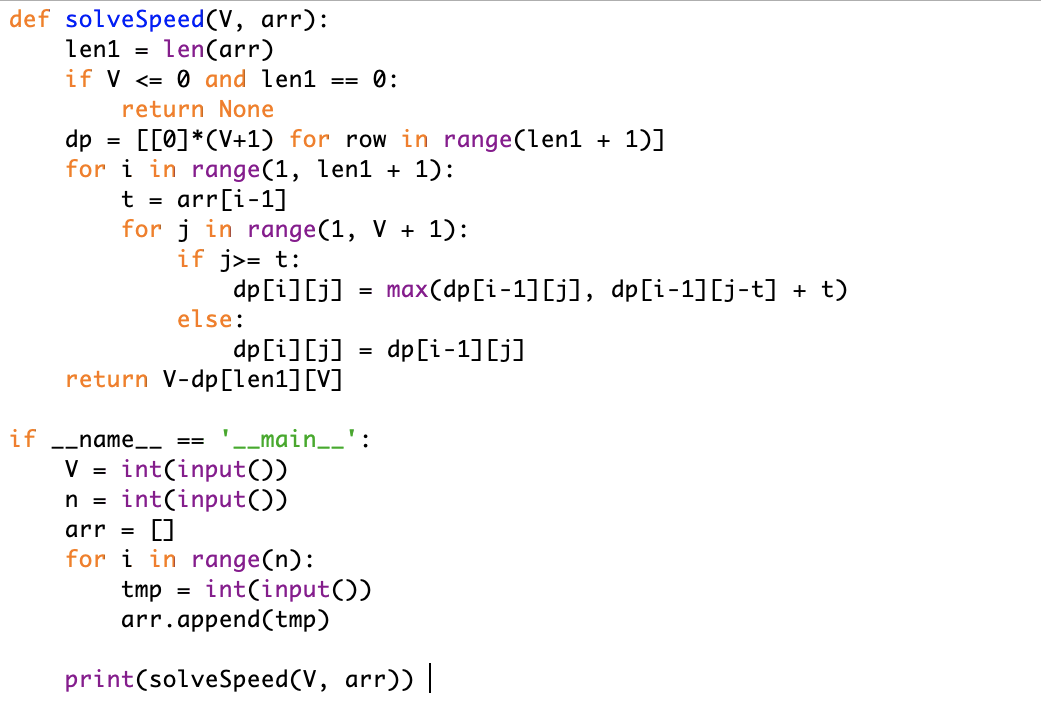
\includegraphics[scale = 0.6]{code2.png}
\end{itemize}
\newpage

\begin{center}
	
	参考文献\\
	
\end{center}
\begin{flushleft}
	[1] 卓金武,李必文,等.MATLAB 在数学建模中的应用[M].北京:北京航空航天大学出版社,2011.

	[2] 杨桂元,朱家明.数学建模竞赛优秀论文评析[M].中国科学院大学出版社,2013.
	
	[3] 程理明,等.运筹学模型与方法教程[M].北京:清华大学出版社,2000.
	
	[4] 刘志华,唐晓强邵珠峰等. 6自由度索并联机构的振动特性[J].机械工程学报,2013,49(3).
	
	[5] 郑亚青. 绳牵引并联机构若干关键理论问题及其在风洞支撑系统中的应用研究[D].华侨大学,2004.
	
    [6] 刘鹏. 柔索牵引并联机器人力学分析及稳定性评价[D].西安电子科技大学,2015.
\end{flushleft}

\end{document} 
